\chapter{Clustering}
We continue to tal about Unsupervised Learning, and in particular about \textbf{Clustering}. We have seen how the \(k\)-means algorithm as one of the simplest algorithm for finding some structure on our training data, in particular to discover groups of similar samples in our set.

When we have our row data we need to extract the features from them, now with the features of the data, we need to group them into clusters. Note that there is \textbf{no supervision}, this means that we are only given data and want to find the groupings of this data.

\textbf{Clustering} is the process of grouping a set of objects into classes of similar objects.

\section{\(k\)-Means}
One of the questions that we want to discuss is \emph{"What algorithm should we choose for clustering?"}, we have already seen the \(k\)-means algorithm, but let's discuss its issues and its properties.

The \(k\)-means is the most popular clustering algorithm with a simple implementation. It starts by initializing randomly the centers, and then it iterate the clustering operation: it clusters each example to the closest center and recalculate centers as the mean of the points in a cluster. 

\subsection{Issues}
\(k\)-means is a very powerful algorithm, however it has some issues, for instance is the calculation of the distance that is done with the euclidean distance
\begin{equation}
    d(x,y) = \sqrt{\sum_{i=1}^n (x_i - y_i)^2}
\end{equation}
However for some applications the euclidean distance could be not the best choice. Let for instance consider the clustering of documents: we have one feature for each word, the value is the number of times that word occurs, and documents are points or vectors in the space. 

\begin{figure}[h!]
    \centering
    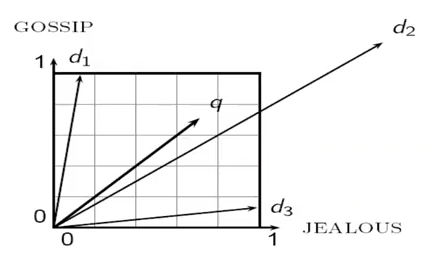
\includegraphics[width=.5\textwidth]{074}
    \caption{Document clustering representation.}
    \label{fig:074}
\end{figure}

With respect to Figure~\ref{fig:074}, which document is closes to \(q\) using the euclidean distance? With the euclidean distance it will be closer to \(d_1\) and \(d_3\), but in practice it should be closer to \(d_2\), because the distributions of the words "GOSSIP" and "JEALOUS" are very similar.

\subsubsection{Distance}
In this case it could be more meaningful to have a different distance, in particular measure the \textbf{cosine similarity} and measure the distance as the difference of the cosine similarity.

The cosine similarity between vectors is correlated with the angular distance between two vectors, and it can be computed in this way:
\begin{equation}
    sim(x,y) = \frac {x \cdot y} {|x||y|} = \frac x {|x|} \cdot \frac y {|y|} = \frac {\sum_{i=1}^n x_iy_i} {\sqrt{\sum_{i=1}^n x_i^2} \sqrt{\sum_{i=1}^n y_i^2}}
\end{equation}

The cosine similarity ranges from 0 to 1, it is good for text data and many other real-world data sets, and it is computationally friendly since we only need to consider features that have non-zero values for both examples.

The cosine distance can be computed as follows:
\begin{equation}
    d(x,y) = 1 - sim(x,y)
\end{equation}

\subsection{Properties}
We already said that the algorithm is guaranteed to converge, because it strictly improves the objective if there is at least a cluster change and the set of possible partitions is finite. It is not guaranteed to find the global minimum (optimum) but a local one.

Regarding to the first property, each step of \(k\)-means move towards reducing the loss function (or at least not increasing it). In the first step (assignment), any other assignment would end up in a larger loss, while in step 2 (centroid computation), the mean of a set of values minimizes the squared error.

Regarding to the second property, it is important to remark that the \(k\)-means loss function is generally not convex and for most problems it has many minima, we are guaranteed to find one of them, but not necessarily the global minimum --- the minimum we find depends on the initialization.

Centroids selection plays an important role with the result, results can vary drastically based on random seed selection, ome seeds can result in poor convergence rate or convergence to sub-optimal clustering. Some common heuristics are:
\begin{itemize}[topsep={0pt}, partopsep={0pt}]
    \itemsep0pt
    \item Random points (not examples) in the space;
    \item Randomly pick examples;
    \item Points least similar to any existing center (furthest centers heuristic);
    \item Try out multiple starting points;
    \item Initialize with the results of another clustering method.
\end{itemize}

\section{Issues for Clustering}
The second question we are interested in discussing is \emph{"What are some of the issues for clustering?"}. In this section we are going to examine some issues that are beyond the \(k\)-means algorithm but still related to the clustering algorithms.

The first issue that we have for clustering is how to represent our data points, we will see that the feature extraction algorithm plays a crucial role. A second thing that we already discussed is that the way we choose to measure the distance between examples in the training set has a strong impact on the final performance of the clustering algorithm. Then, another issue is if the problem necessitates flat clustering or hierarchical clustering algorithms. A final factor that we need to discuss is how to define the number of cluster we are going to consider in our dataset, number of cluster can be fixed a priori or data driven.

\subsection{Types of Clutering Algorithms}
Clustering algorithms can be devided in\textbf{Flat Algorithms} and \textbf{Hierarchical Algorithms}. Flat algorithms usually start with a random partial partitioning and refines it iteratively (e.g. \(k\)-means and model based clustering). Hierarchical algorithms are bottom-up agglomerative (progressively aggregate data) or top-down divisive (split the dataset).

Regarding flat algorithms, flat clustering algorithms can be implemented in two ways: \textbf{Hard clustering}, where each example belongs to exactly one cluster (e.g. \(k\)-means); and \textbf{Soft clustering}, where an example can belong to more than one cluster (probabilistic). Soft clustering makes more sense for applications like creating browsable hierarchies, suppose for example you want to put a pair of sneakers in two cluster (sports apparel and shoes), then soft clustering is required.

\section{EM Clustering}
The \(k\)-means algorithm we have seen assumes spherical clusters, this means that a sub-optimum solution can be like the one in Figure~\ref{fig:075}, that we can see is not the optimal solution. 

The improved version of \(k\)-means it's called \textbf{EM Clustering} and assumes that data came from a mixture of Gaussians (elliptical data), assigns data to cluster with a certain probability (soft clustering). In Figure~\ref{fig:076} we can see that it provides a better clustering solution for our dataset.

\begin{figure}[t!]
    \centering
    \begin{subfigure}{.4\textwidth}
        \centering
        \label{fig:075}
        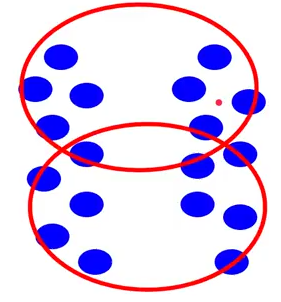
\includegraphics[width=.75\textwidth]{075}
        \caption{Spherical clusters}
    \end{subfigure}
    \begin{subfigure}{.4\textwidth}
        \centering
        \label{fig:076}
        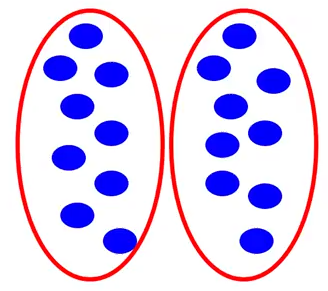
\includegraphics[width=1\textwidth]{076}
        \caption{Elliptic clusters}
    \end{subfigure}
    \caption{Spherical clusters vs. Elliptic clusters.}
\end{figure}

The idea of EM clustering is to follow an iterative scheme as \(k\)-means, it iterates between assigning points and recalculating cluster centers. The two main differences between \(k\)-means and EM clustering are:
\begin{itemize}[topsep={0pt}, partopsep={0pt}]
    \itemsep0pt
    \item We assume elliptical clusters instead of spherical clusters.
    \item It is a soft clustering algorithm.
\end{itemize}

\subsection{Soft Clustering in EM Clustering}
EM clustering is a soft clustering algorithm, this means that is a probabilistic algorithm. In order to understand more the meaning of \emph{probabilistic}, let's take as an example the dataset in Figure~\ref{fig:076}: given a point \(\vec{d}\) in the right-side ellipse, \(\vec{d}\) has a certain probability to be \(right\) (e.g. \(p(right) = 0.8\)), and another probability to be \(left\) (e.g. \(p(left) = 0.2\)); this means that it is assigned to a cluster based on the highest probability to be of one of the clusters, in this case it is the left cluster.

\subsubsection{EM Algorithm}
EM algorithm operate in this way:
\begin{algorithm}
    \caption{EM Clustering}
    \label{alg:em_clustering}
Initialize clusters\;
\While{clusters does not change}{
    Calculate \(p(\Theta_c | x)\) the probability of each point belonging to each cluster\;
    Recalculate the new cluster parameters \(\Theta_c\), the maximum likelihood cluster centers given the current soft clustering\;
}
\end{algorithm}

\begin{figure}[t!]
    \centering
    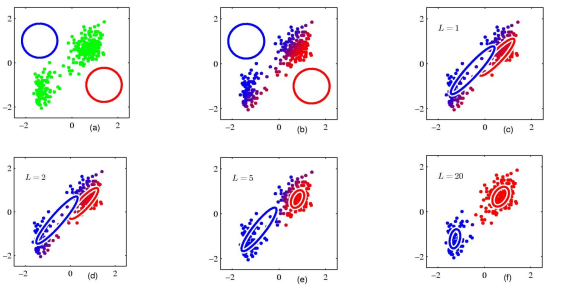
\includegraphics[width=.75\textwidth]{077}
    \caption{EM Clustering Algorithm execution example.}
    \label{fig:077}
\end{figure}

\subsection{Mixture of Gaussians}
We have seen the intuition of the EM clustering, but we have not seen how do we define a Gaussian (i.e. ellipse), this requires a bit of math.

In the case of one dimensional distributions, the gaussian is parametrized by the mean and the standard deviation/variance:
\begin{equation}
    \label{eq:001}
    f(x; \sigma, \Theta) = \frac 1 {\sigma \sqrt{2\pi}} exp\left\{ - \frac {(x-\mu)^2} {2\sigma^2} \right\}
\end{equation}

The equation can be extended in an \(m\)-dimensional space, where the gaussians are calculated as follows:
\begin{equation}
    N[x; \mu, \Sigma] = \frac 1 {\sqrt{(2\pi)^d} \sqrt{det(\Sigma)}} exp \left\{ - \frac 1 2 (x - \mu)^T \Sigma^{-1} (x - \mu) \right\}
\end{equation}
where \(\Sigma\) is the covariance matrix, and we have one gaussian for each cluster. Given the Algorithm~\ref{alg:em_cluster}, the second step inside the iteration, the cluster parameters will be the mean vector and the covariance matrix that better fit the assigned clusters. In \(m\)-dimensional space we learn the means of each cluster (i.e. the center) and the covariance matrix (i.e. how spread out it is in any given direction).

\subsection{Expectation Maximization}
EM stands for Expectation Maximization:
\begin{itemize}
    \item[Expectation:] Given the current model, figure out the expected probabilities of the data points to each cluster \(p(\Theta_c | x)\). \emph{"What is the probability of each point belonging to each cluster?"}.
    \item[Maximization:] Given the probabilistic assignment of all the points, estimate a new model \(\Theta_c\). \emph{"Maximum likelihood estimation"}.
\end{itemize}

EM is similar to \(k\)-means, each iteration increases the likelihood of the data and is guaranteed to converge (though to a local minimum). EM is a general purpose approach for training a model when you don't have labels, but it is not just for clustering (while \(k\)-means is just for clustering).

\section{Other Clustering Algorithms}
\(k\)-means and EM clustering are by far the most popular clustering algorithms. However, they cannot handle all clustering tasks. As an example, let's consider the example in which we have non-gaussian data --- i.e. in Figure~\ref{fig:078} we have two circles and two clusters with \(k\)-means, but it is obviously an incorrect solution.

\begin{figure}[h!]
    \centering
    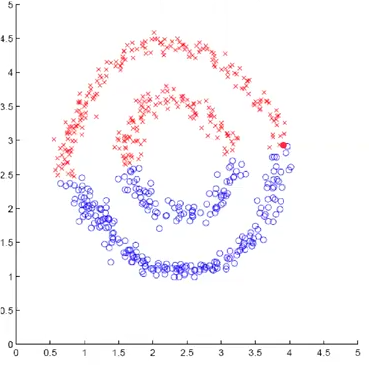
\includegraphics[width=.5\textwidth]{078}
    \caption{Two circles and two clusters (\(k\)-means).}
    \label{fig:078}
\end{figure}

\subsection{Spectral Clustering}
The idea of spectral clustering methods is represented in Figure~\ref{fig:079}, where we form a matrix that indicate the similarity of each data point with respect to each other.

\begin{figure}[h!]
    \centering
    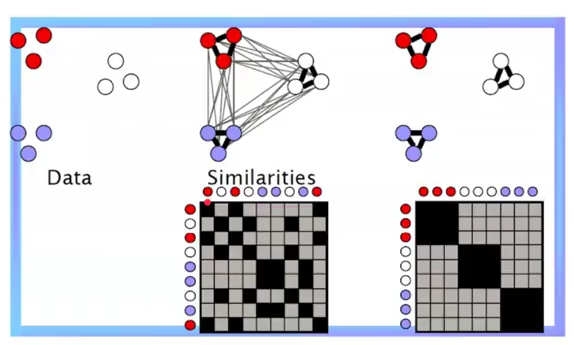
\includegraphics[width=.5\textwidth]{079}
    \caption{}
    \label{fig:079}
\end{figure}

This similarity matrix can be also represented in term of graphs, where each edge indicates the similarity between two points. The black edges in the adjacent matrix, that are harder edges in the graph, are called high similar points. If we cut the lowest similar edges, we have then our high-similar clusters.

\subsection{Hierarchical Clustering}
The last family of clustering algorithm we are going to discuss is the family of \textbf{Hierarchical Clustering Algorithm}, that are perceived for flat solution. 

Hierarchical clustering algorithms produce a set of nested clusters organized as a hierarchical tree. The tree is called a \textbf{dendogram}.

\begin{figure}[h!]
    \centering
    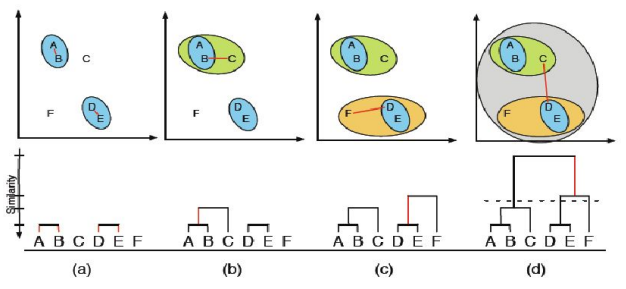
\includegraphics[width=.75\textwidth]{080}
    \caption{Hierarchical Clustering Dendrogram example.}
    \label{fig:080}
\end{figure}